% This document is part of the EPRVCalibration project
% Copyright 2019 the authors. All rights reserved.

% style notes
% -----------
% - use \acronym and use \eprv, \lfc, and so on.

\documentclass[12pt, letterpaper]{article}
\usepackage{xcolor}
\newcommand{\lz}[1]{\textcolor{orange}{#1}}

\usepackage[ruled,vlined]{algorithm2e}
\usepackage{graphicx}

% typesetting words
\newcommand{\project}[1]{\textsl{#1}}
\newcommand{\name}{\project{Excalibur}}
\newcommand{\acronym}[1]{{\small{#1}}}
\newcommand{\expres}{\project{\acronym{EXPRES}}}
\newcommand{\eprv}{\acronym{EPRV}}
\newcommand{\lfc}{\acronym{LFC}}

% math shih
\newcommand{\mps}{\mathrm{m\,s^{-1}}}

% margins and page setup, etc
\addtolength{\textheight}{1.00in}
\addtolength{\topmargin}{-0.50in}
\sloppy\sloppypar\raggedbottom\frenchspacing

\begin{document}

\section*{\raggedright%
\name:
A non-parametric, hierarchical model for a precision spectrograph}

\noindent
\textbf{Lily~Zhao} (Yale) (Flatiron),
\textbf{David~W~Hogg} (NYU) (MPIA) (Flatiron),
\ldots and others\ldots

\paragraph{Abstract:}
There have been many hardware improvements in polygonal-fiber-fed,
temperature-controlled, laser-frequency-comb or etalon-calibrated,
high-resolution, extreme-precision radial-velocity spectrographs.
Have the calibration methodologies improved to match?
Here are three relevant observations:
The first is that the calibration lines or spots from an etalon or
comb (or even arc lamp) fill the spectral range with dense calibration points.
The second is that the spectrograph lives in a stabilized,
climate-controlled environment, in which the full optical system and
detectors will only vary within a tiny range of configurations or
settings.
The third is that, given this stability, every calibration image
ever taken is relevant to every science exposure ever taken; there is
no reason to calibrate every exposure independently.
The calibration methodology we propose here---\name---addresses these
three problems by going non-parametric (no more polynomials!) and then
reducing dimensionality with a robust principal-component method.
We demonstrate the success of this method with comb and arc data
from the \expres\ spectrograph.
We find... [results and so on].

\section{Introduction} 

Extreme precision radial-velocity (\eprv) programs have been
outrageously successful in finding and characterizing extra-solar
planets (CITE THINGS).
These programs typically make use of spectrographs with resolutions on
the order of $10^5$, which correspond to line widths on the order of
$3000\,\mps$.
Exoplanet science happens at $3\,\mps$ precisions, and the current
instruments hope to get to $0.1\,\mps$ precisions (CITE THINGS).
This means that new spectrographs are expected to be calibrated or
stabilized to better than $10^{-4}$ of a pixel (assuming that the
spectrograph is well sampled).
And indeed, some hardware--software systems seem to be reaching these
levels (CITE THINGS).

Here we propose to simplify and improve calibration programs for
\eprv\ hardware systems with two very simple but novel ideas.
The first flows from the observation that calibration sources---which
include lamps, etalons, and laser-frequency combs (\lfc
s)---illuminate the spectrograph with dense sets of lines; almost every
location in the spectrograph image plane is surrounded by nearby,
useful calibration lines.
This recommends a calibration methodology that is
\emph{non-parametric}:
If every point in the spectrograph detector is surrounded by nearby
calibration lines, the wavelength solution can be made simply an
interpolation of the calibration data.
There is no need to choose any functional form for the wavelength
solution (such as an eighth-order polynomial, for example).
Going non-parametric will improve calibration accuracy, because
choosing a parametric form biases the calibration, and biases it
badly when the form is inappropriate (as, for example, polynomials
will be at the detector edges).

The second idea here flows from the observation that contemporary
\eprv\ instruments are incredibly stable.
Temperature-controlled, fiber-fed pectrographs vary only slightly over
the night or season, and only along a small number of axes in what you
might call ``calibration space'', or the (very high dimensional) space
of all possible wavelength solutions.
That is, not only are they stable, but they don't have many accessible
degrees of freedom.
So it is not appropriate to fit each calibration exposure or calibrate
each science exposure independently.
It makes sense to use the calibration data (or all the data) to
determine the space in which the instrument can and does vary, and
then in subsequent calibration work only permit the solution to live
in the accessible part of calibration space.
This structure is \emph{hierarchical}: The calibration data are used
not just to determine the wavlength solution, but also to determine
the possible space of wavelength solutions.
In the statistics literature this concept is often described as
\emph{de-noising}:
Every calibration exposure contains information about every other
exposure; it doesn't just constrain the instrument locally in time.
Thus every exposure can be improved (de-noised) with information
coming from every other exposure.

The method we propose here---\name---embodies these ideas.
It is a non-parametric, hierarchical, data-driven model for the
wavelength solution.
By being non-parametric, it delivers enormous freedom to the
wavelength solution to match or adapt to any instrument or detector
oddities.
By being hierarchical, it restricts that freedom tremendously, but it
does so appropriately for the observed variations in the
spectrograph.
\name\ is designed for temperature-controlled, bench-mounted, fiber-fed
spectrographs with good calibration sources, such as laser-frequency
combs, etalons, or good arc lamps.
We have in mind the \eprv\ instruments and \eprv\ science cases.
But we expect \name\ to have applications for other kinds of
spectrographs in other contexts; the motivating ideas behind this
project are true for almost every astronomical spectrograph.

\section{Method} \label{sec:method}
We operate on the two core ideas that the wavelength solution should be given enormous flexibility, but that in fact it will be living in a very low-dimensional space, where the degrees of freedom are set by the limited kinematics of the spectrograph hardware.

We will pose the problem in the following way.  Given an exposure $n$, and order $m$, there is a relationship between
the two-dimensional $(x,y)$-position on the detector and the
wavelength $\lambda$
\begin{equation}
\lambda(x,y,m,n) = f(x,y,m;\theta_{n})
\quad ,
\end{equation}
where $\theta_{n}$ is a big blob of parameters for this exposure.

A stabilized spectrograph should experience only low-degree variability, meaning the calibration of any image can be informed by the calibration of every other image.  To implement such a hierarchical model, we use the calibration data themselves to develop a low-dimensional basis for expressing the calibration data.

If the space of all calibration possibilities is in fact $K$-dimensional (where K is a small integer, i.e 2 or 8 or thereabouts), and if the calibration variations are so small that we can linearize, then the function $f(x,y,m;\theta_{n})$ could be replaced with a tiny model
\begin{equation}
\lambda(x,y,m,n) = g_0(x,y,m) + \sum_{k=1}^K a_{nk}\,g_k(x,y,m)
\quad ,
\end{equation}
where
$g_0(x,y,m)$ is the fiducial or mean or standard calibration of the spectrograph,
the $a_{nk}$ are scalar amplitudes,
and the $g_k(x,y,m)$ are basis functions expressing the ``directions'' in calibration space that the spectrograph can depart from the fiducial calibration.

The challenge is to learn these basis functions from the data and get the $K$ amplitudes $a_{nk}$ for every exposure $n$.  There are many ways to discern these basis functions.  Here, we present a model using principal component analysis (PCA).  This is the correct thing to do in the limit where we have very high SNR, as is undeniably the case with calibration images.

\subsection{Data} \label{sec:data}
We present results using data from \expres\, the EXtreme PRecison Spectrograph.  \expres\ is an environmentally-stabilized, fiber-fed, $R\sim137,000$, optical spectrograph (\lz{CJ and RB's papers}).  \expres\ has two different wavelength calibration sources, a ThAr lamp and a Menlo Systems laser frequency comb (LFC, e.g. \lz{Wilken+ 2012, Molaro+ 2013, Probst+ 2014, from RB's paper}).  ThAr exposures are taken at the beginning and end of each night.  LFC exposures are interspersed between science exposures every ~15 minutes.

The method and results discussed here are based off of 1260 LFC exposures and ThAr exposures over 90 days.  Exposures were taken whenever EXPRES was assigned time and so are randomly distriubted throughout the nine days

\lz{(Discussion of number of orders covered or number of lines in LFC and/or ThAr?)}

For the results presented in this paper, we work with the 1D, optimally extracted data.  This removes the y-dependence from equations 1 and 2.  Gaussian profiles are fit to each line in the 1D, extracted data.  The mean of each fitted Gaussian is taken to be the center of the line.  This process is described in detail in \lz{RP Paper} and considered out of scope of this paper.  The method described proceeds from a given list of orders, line wavelengths, and line centers for each exposure.

\expres\ exposures are separated into different ``instrumental epochs," which correspond to atypical, large instrument changes that affected the position of the echellogram on the detector, the shape of the instrumental PSF, or the calibration sources (\lz{can cite either Ryan's paper for more detail?}).  Because significant instrumental changes break the assumption of only low-dimensional variations in the spectrograph hardware, we treat each instrument epoch independently.

\subsection{Hierarchical De-Noising of Calibration Frames} \label{sec:denoising}
Let $\{exp_n\}$ be the set of calibration exposures within an instrument epoch.  These are the exposures to be used in constructing $g_k(x,y,m)$.  We first identify the full list of lines we can expect to find in a calibration image from this epoch.  A line is uniquely defined by a combination of order, $m$, and ``true" or theoretical wavelength of that line, $\lambda$.  We define $\{l_{m,\lambda}\}$ to be the complete list of unique lines found in $\{exp_n\}$.

For each line, $l_{m,\lambda}$, we then find the fitted line center, $x_{n,l}$, in pixel space, for that line in each calibration exposure.  If this line is missing from an exposure (e.g. it was covered by noise or off the edge of its usual order), we insert a $NaN$ for that line center instead.

Lines that are missing from greater than some percent of exposures are completely cut from the analysis.  Exposures that are missing greater than some percent of lines are also cut.  We use a threshold percentage of 50\% for both lines and exposures.  This largely affects the first lines on either end of an order and exposures with spuriously low signal.  Typically, about 0.2\% of lines and cut for LFC based calibration and 0.25\% of files are cut.

Missing line center measurements are replaced with denoised estimates using iterative PCA.  For each missing line center measurement, we initialize their value to the mean of the nearest $n$ exposures in time, where $n$ is typically $9$ exposures.  We then find a fiducial calibration of the spectrograph,  $g_0(x,y,m)$, for which we use the mean line center value for each identified line.  We subtract this fiducial calibration from each exposure's measured line centers and run PCA on the difference between the measured and mean line center for each exposure.  This process gives us $a_{nk}$ and $g_k(x,y,m)$.

Using those values with equation 2 and some small integer (e.g. 2) for $K$, we can reconstruct a de-noised matrix of line centers for each exposure.  Missing line center measurements are replaced with values from this reconstruction.  We iterate until the values of the missing line centers change by less than 0.01\% of a pixel.  This convergence suggests that the PCA is no longer being swayed by outliers and is truly ``de-noised."

\begin{algorithm}
\SetAlgoLined
\textbf{Inputs}: ${m,\lambda}$, $\{l_{m,\lambda}\}$ \;
\While{change in bad lines $>$ 0.01\%}{
	$g_0(x,y,m) = \overline{\{x_{n,l}\}}$\;
	find $U, \Sigma, V$ s.t. $U\Sigma V^* = (x_{l,n}-g_0(x,y,m))$\;
	let $a_{n,k} = U\cdot \Sigma$ and $V = g_k(x,y,m)$\;
	$\lambda(x,y,m,n) = g_0(x,y,m) + \sum_{k=1}^K a_{nk}\,g_k(x,y,m)$ where $K=2$\;
	$\{x_{n,l}\} = \lambda(x,y,m,n)$ where $\{x_{n,l}\}$ was initially $NaN$
	}
\caption{Hierarchical De-Noising}
\end{algorithm}

Following the de-noising process, we check for deviant line centers.  This is aimed at catching lines that have been mis-identified or poorly fit, resulting in erroneous line centers.  Outliers are identified via a simple sigma cut for each line.  Any line center that is reported at more than $3\sigma$ away from the mean line center value is relabeled a ``bad line,'' and we repeat the process of hierarchical de-noising. (\lz{Should probably add something about why the sigma cut works})

\subsection{Non-Parametric Calibration} \label{sec:nonparam}
The process of hierarchical de-noising gives us $a_{nk}$, which captures the variability of the instrument.  We can interpolate $a_{nk}$ with respect to housekeeping data to determine $\lambda(x,y,m,n)$ at any time.  In this paper, we show results where $a_{nk}$ is interpolated with respect to time, but it is possible to incorporate other information such as temperature, pressure, or telescope position. (\lz{Does this belong in the discussion?})

Once we have the line center for every line in $\{l_{m,\lambda}\}$, each of which is associated with a known wavelength, we can interpolate the known wavelengths over line centers to any position in x in a given order.  For example, interpolating onto every integer x will generate wavelengths for each pixel in an order.

\begin{algorithm}
\SetAlgoLined
\textbf{Inputs}: new time, new line centers, new orders\; %command not working for w/e reason
Let $t_n$ be the time associated with exposure $n$\;
let $t_n'$, $x_n'$, and $m_n'$ be the new time, line centers, and orders we want wavelengths for\;
Let $a_{n,k}'$ be the interpolation of $a_{n,k}$ to time $t_n'$\;
$\lambda(x,y,m,n)' = g_0(x,y,m) + \sum_{k=1}^K a_{nk}'\,g_k(x,y,m)$ where $K=2$\;
\For{each unique $m_n'$}{
	${l_n,m}$ from $\lambda(x,y,m,n)'$
	interpolate ${l_n,m}$ onto $x_n'$\;
	}
\caption{Non-Parametric Wavelength Solution}
\end{algorithm}
\lz{What's fancy math symbol for interpolate?}

\subsection{Choice Choices} \label{sec:choices}
Implementing \name required choosing some global variables and methods that we believe is optimal for constructing a high-fidelity wavelength solution.  We discuss these choices here and how we came to each decision.

\subsection{Value of K}
The value of $K$ determines how many principal components are used to reconstruct de-noised line centers.  This $K$ needs to be large enough that all variability in the spectrograph is captured.  Too large, and the reconstruction will begin to incorporate noise, defeating the purposes.

We settled on a $K$ value of 2.  Figure \ref{fig:eigenvectors} shows the eigenvectors of the PCA plotted on a log scale for both a LFC-based calibration scheme (blue), and a ThAr-based one (green).  In both cases, there is a precipitous drop off at one, indicating that the later principal components have a much smaller contribution.

\begin{figure}[h]
\centering
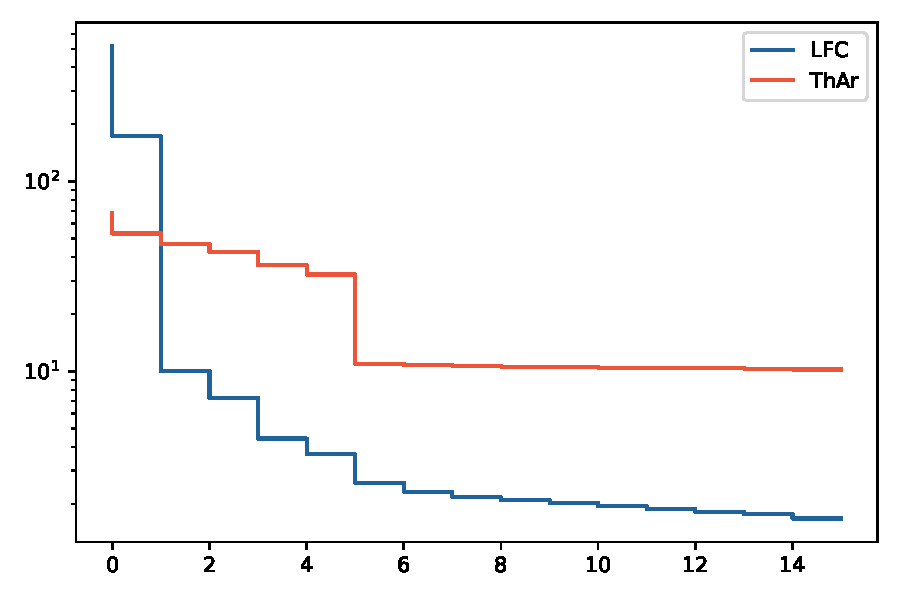
\includegraphics[width=0.5\textwidth]{Figures/ss.pdf}
\caption{Eigenvectors from PCA as step functions.  The results for using only LFC exposures (blue) and only using ThAr exposures (green) are both shown on a log scale.  After 1, there is a order of magnitude drop for both the LFC and the ThAr.}
\label{fig:eigenvectors}
\end{figure} 

Figures \ref{fig:pcLfc} and \ref{fig:pcThar} shows the first 6 principal components for the LFC and ThAr respectively.  In both cases there is clear structure in the first and second principal components.  It is doubly encouraging that this structure appears the same in both the case with the LFC and the ThAr.

The later principal components show mostly noise or are swayed by large noise sources.  For example, the band on the left side of each order in principal component 3 for the LFCs is likely due to lower signal on the edges of the order from the blaze function, giving more uncertain line center measurements.  The diagonal banding visible in the sixth principal component can be traced to what we believe are detector defects.

\begin{figure}[t]
\centering
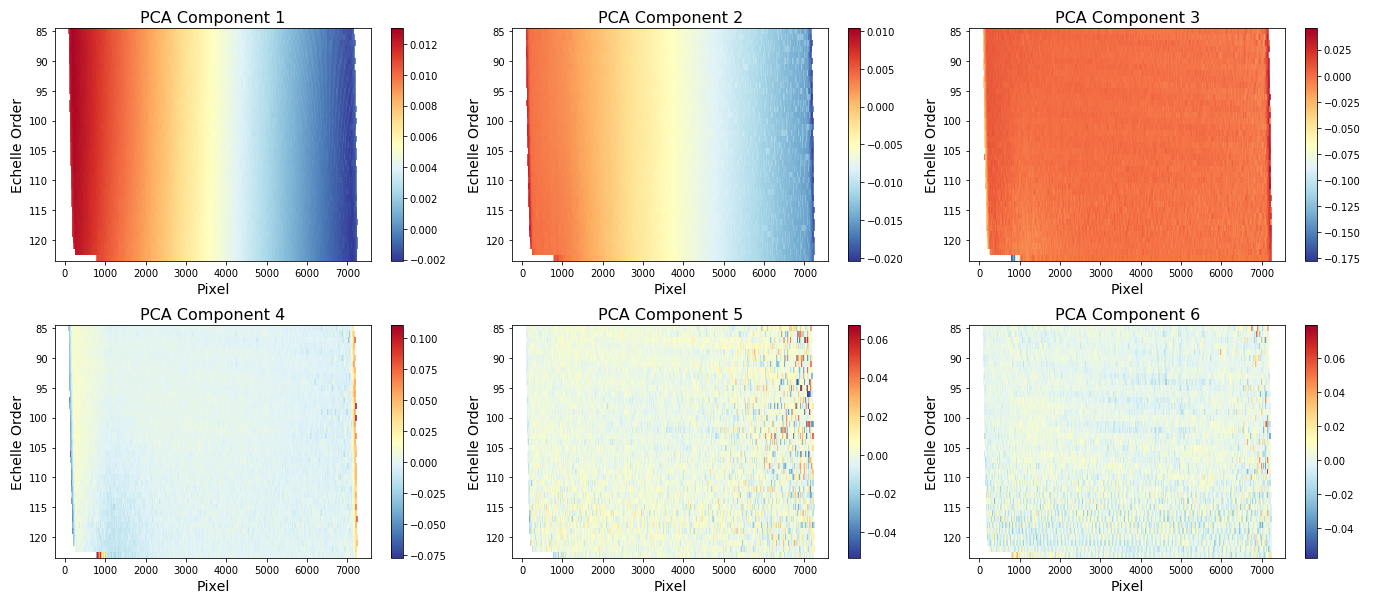
\includegraphics[width=\textwidth]{Figures/pcsLfc6.png}
%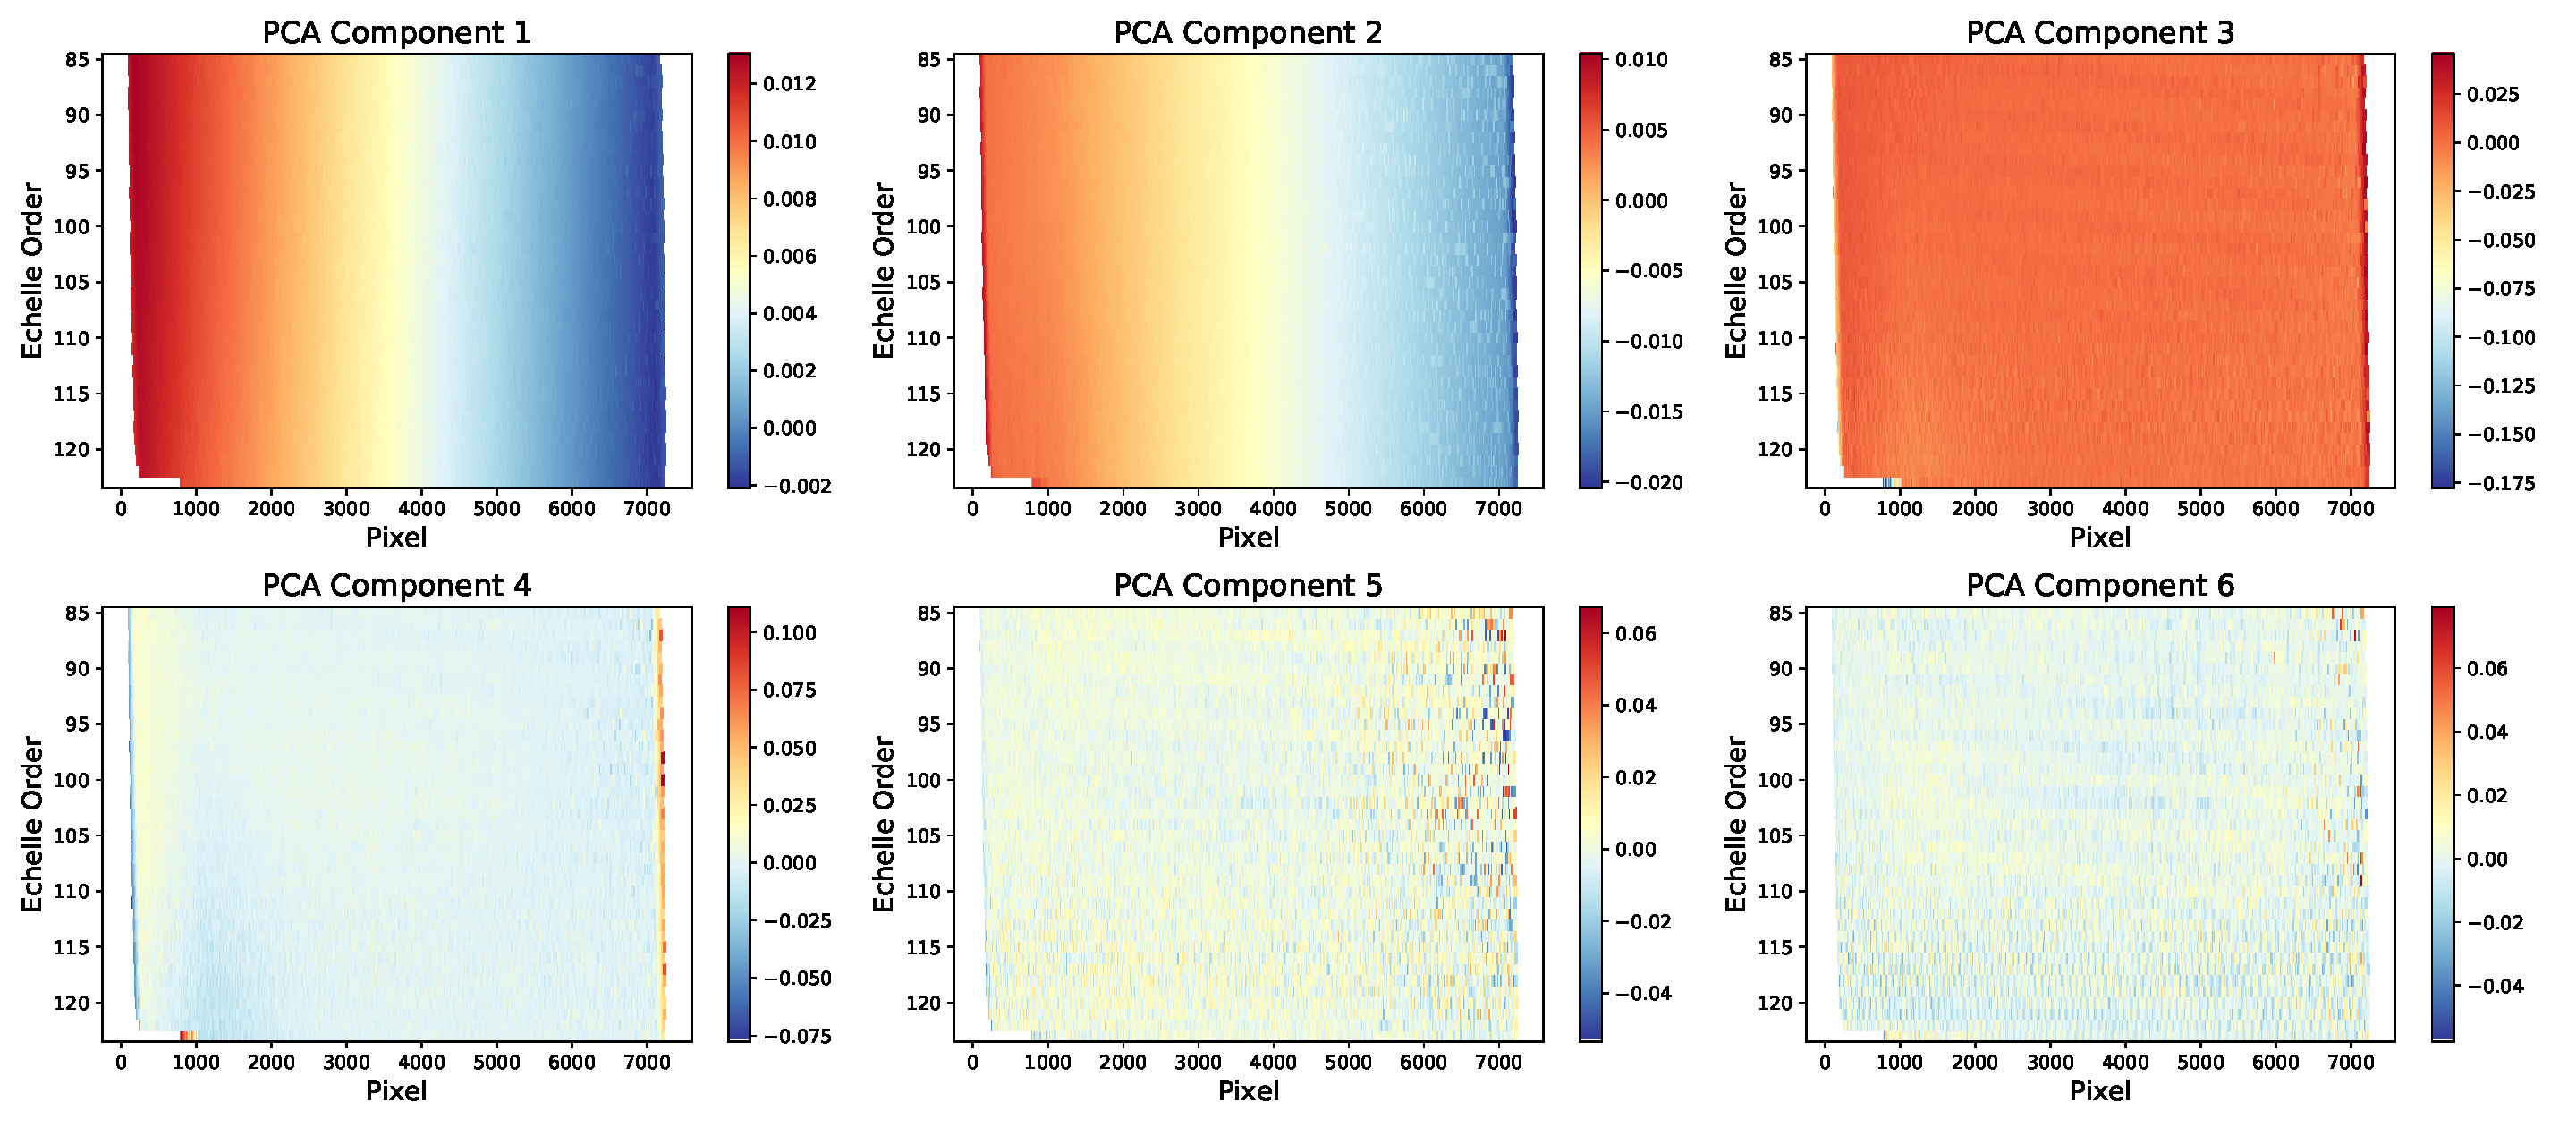
\includegraphics[width=\textwidth]{Figures/pcsLfc6.pdf}
\caption{The first six principal components using LFC exposures.  There is clear structure for the first two principal components.  \lz{Principal components 3-5 show mostly noise (do they though?)}.  Principal component 6 shows structure from what we believe to be detector defects.}
\label{fig:pcLfc}
\end{figure}

\begin{figure}[t!]
\centering
\includegraphics[width=\textwidth]{Figures/pcsThar6.png}
%\includegraphics[width=\textwidth]{Figures/pcsThar6.pdf}
\caption{The first six principal components using ThAr exposures.  Note the similarities with the LFC result shown in Figure \ref{fig:pcLfc}.}
\label{fig:pcThar}
\end{figure}

\subsection{Interpolation in Time}
Figure \ref{fig:nightlyVariation} shows the amplitude of the first and second principal component with respect to time on the left.  Again, it is comoforting to note that the LFC and ThAr versions show the same shape.  Though there are no large trends over the ninety days of data shown here, there is a clear linear trend within each night (see Fig. \ref{fig:nightlyVariation} right).  We therefore interpolate these amplitudes with respect to time using a simple linear interpolation scheme.

\lz{linear interpolation actually doesn't look super great for the second principal component}

\begin{figure}[h!]
\centering
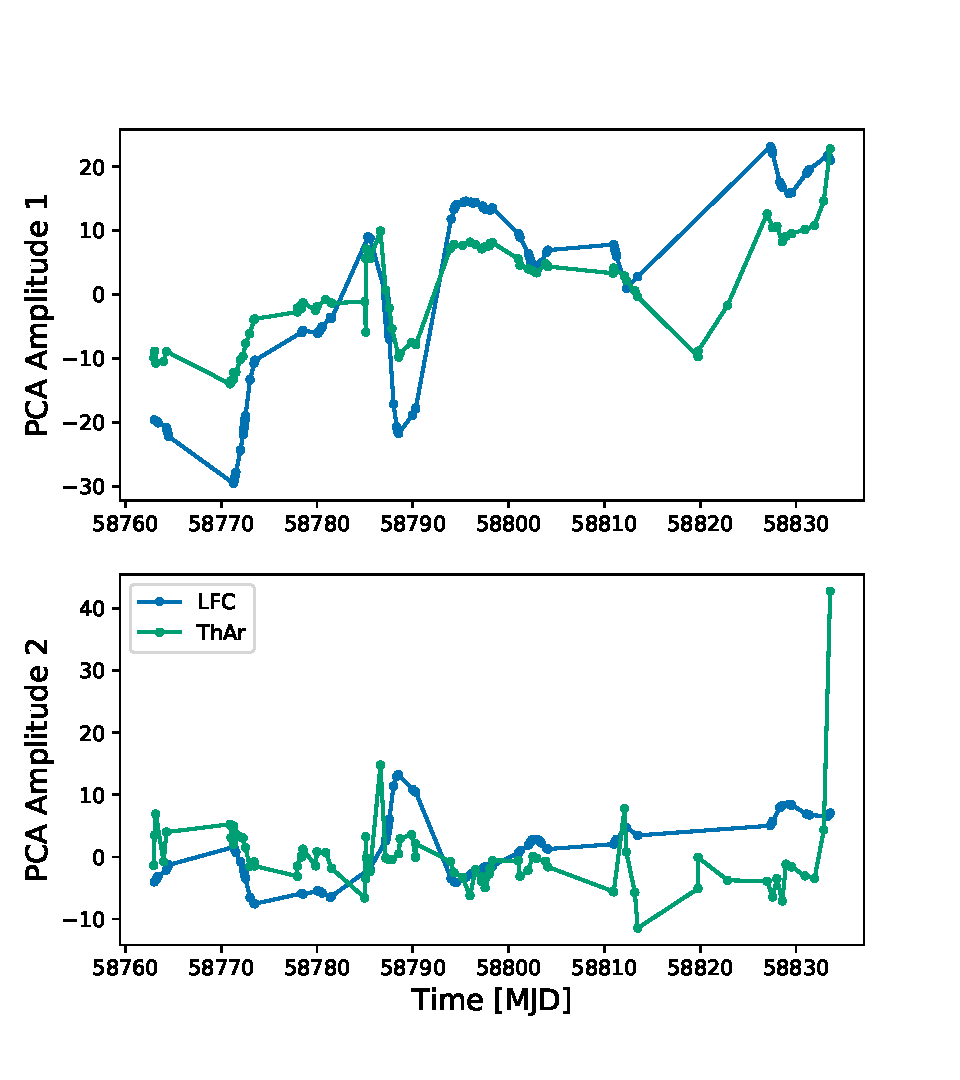
\includegraphics[width=0.56\textwidth]{Figures/pcAs.pdf}
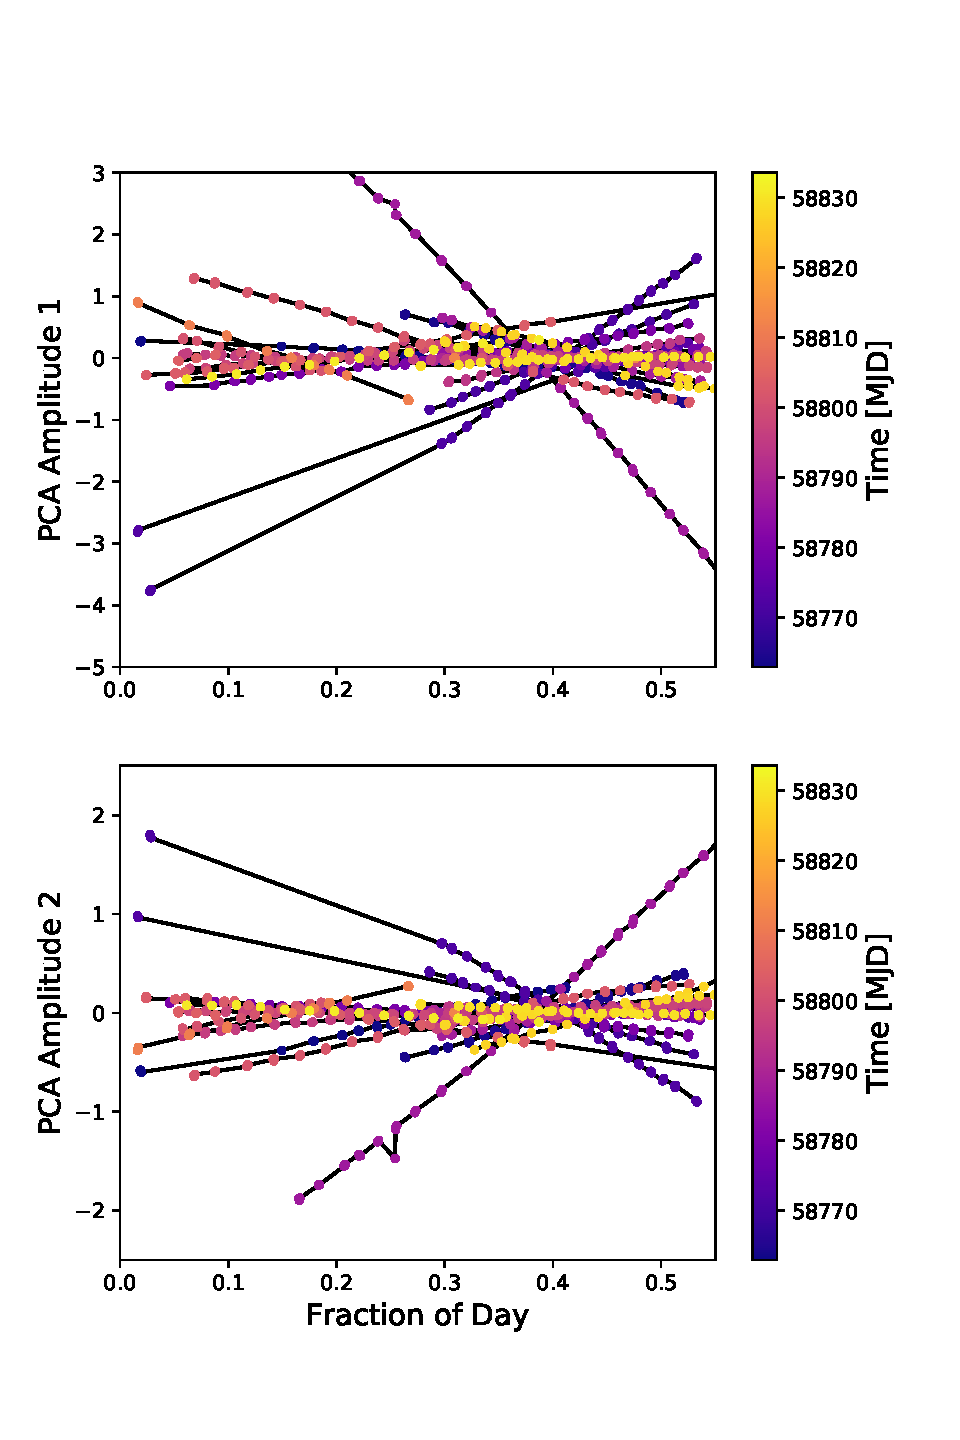
\includegraphics[width=0.42\textwidth]{Figures/pcAs_byDay.pdf}
\caption{Amplitude of the first two principal components show as a function of time (left) or fraction of a day (right).  Points mark the times at which we have calibration data.  Lines show the result of a linear interpolation.  Left: amplitudes as a function of time for both LFC (blue) and ThAr (green).  The top plot shows the amplitudes for the first prinicpal component while the bottom plot shows the amplitudes for the second principal component.  Note that the shape of the curves is similar regardless of calibration source.  Recall from Figures \ref{fig:pcLfc} and \ref{fig:pcThar} that the corresponding principal components are also fairly similar.
Right: amplitudes of the first two principal components determined by the LFC exposures only.  Here exposures are grouped by day and plotted with respect to what time of day the exposure was taken.  A linear interpolation through all the LFC exposures taken in one day are shown as black line.  Points are colored by the MJD of the exposure.}
\label{fig:nightlyVariation}
\end{figure} 

\subsection{Interpolation in Pixel}
Interpolation of wavelengths over line centers is done order by order using a Piecewise Cubic Hermite Interpolating Polynomial (PCHIP) interpolator.  This interpolation incorporates the flexibility needed to model the changing dispersion of the spectrograph across an order while also enforcing monotonicity.

Due to the dispersion intrinsic to echelle spectrographs, the wavelength change between pixels is greater at greater wavelengths.  This means that the function of wavelength given pixel across an order will necessarily be concave down everywhere.  Consequently, linear interpolation of this function will systematically give erroneously low values.

A more classic cubic spline interpolator runs into issues with lines in the ThAr that are blended and therefore very close together.  Very close lines cause huge deviations from the correct wavelengths, as seen in Figure \ref{fig:xinterp}, which highlights deviations caused by a blend in a specific order of ThAr exposures.

\begin{figure}[h]
\centering
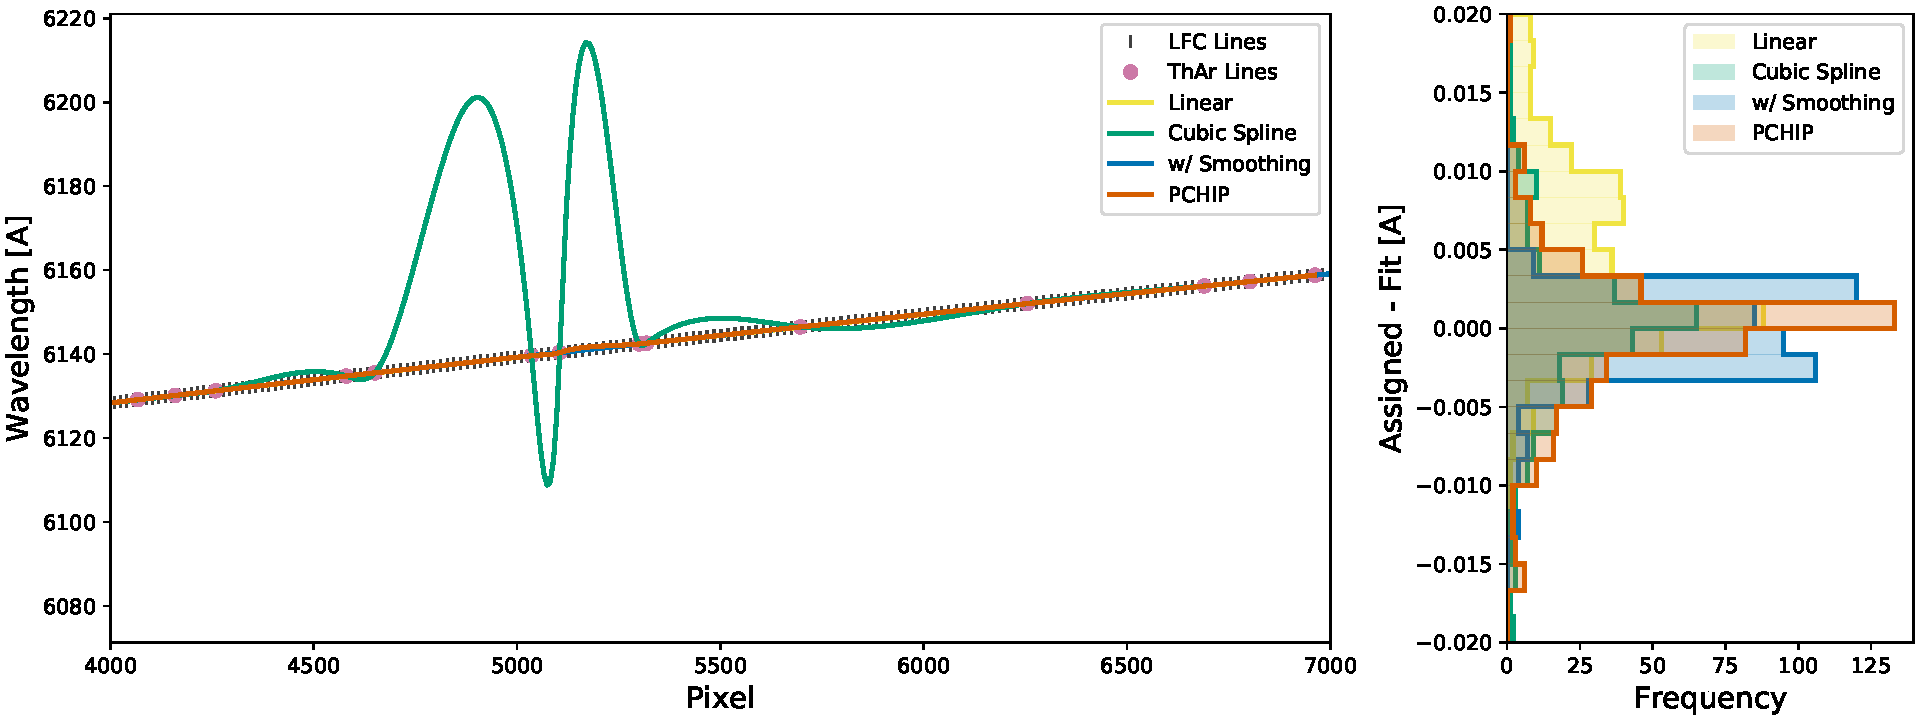
\includegraphics[width=\textwidth]{Figures/intpx_tests.pdf}
\caption{Results from different interpolation schemes in the pixel direction.
Left: resultant wavelength solution curves when using ThAr lines (green points) to predict wavelengths for LFC lines (black points).  The green points are being used to predict values for the black points.  Different interpolation schemes are shown in different colors.  The largest deviation comes with the classic cubic spline (pink).  The other models are hard to distinguish.
Right: histograms of residuals for each method.  The linear interpolation model (yellow) is asymmetric with disproportionately positive residuals.  The classic cubic spline residuals (pink) has very spread out residuals, the extremes of which have been cut off in the figure.  The residuals from an interpolation scheme that incorporates smoothing (blue) are non-Gaussian and rather plateau about zero.  Residuals from the PCHIP interpolator (orange) has the strongest peak at 0 and is roughly Gaussian.}
\label{fig:xinterp}
\end{figure} 

These huge digressions can be avoided by allowing for some smoothing in the interpolation.  In Figure \ref{fig:xinterp}, we show an example in blue using scipy's Univarate Spline method.  While the result appears to follow the calibration lines much better, the smoothing ultimately causes larger residuals that are spatially correlated (Fig. \ref{fig:xinterp}, right).

For all orders, the edges will be overestimated while the middle will be underestimated.  (\lz{Do I need to include a figure for this?  Or should I just not go into this much detail})  This indicates that the smoothing is causing the resultant wavelength solution to underestimate the curvature of the pixel-wavelength relation.  It also reduces the benefit we get from moving to a non-parametric model by enforcing a smoothness we have no reason to believe is true in the data.

We instead turn to the PCHIP interpolator, which damps down huge deviations in the traditional cubic spline by requiring the resulting interpolated function to be monotonic.  This is a constraint we know is true from the optics since interpolation in the pixel direction is carried out order-by-order.  From Figure \ref{fig:xinterp}, it is clear that the PCHIP interpolator returns the lowest residuals.

\subsection{Order of Interpolation}
Now doing time then x direction.  \lz{No real reason for the switch except this makes more sense (well, to me) and is faster.}


\section{Results} \label{sec:results}
\subsection{Self Tests} \label{sec:test-self}
First, let's have a sanity check.  (\lz{Is it worth mentioning this at all?}) Using a linear interpolator with no smoothing, we predict wavelengths for the denoised line center values, $\lambda(x,y,m,n)$, for an exposure used in the training set.  This returns identical values to the assigned true wavelength for each line within machine error for both ThArs and LFCs (see Fig. \ref{fig:sanity test}).

\begin{figure}[h]
\centering
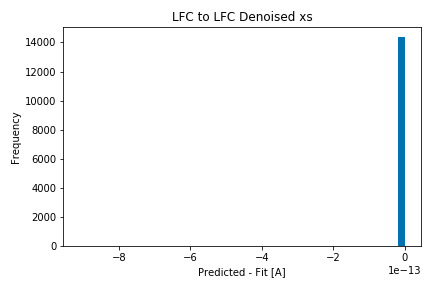
\includegraphics[width=0.48\textwidth]{Figures/lfcLfcDenoised.pdf}
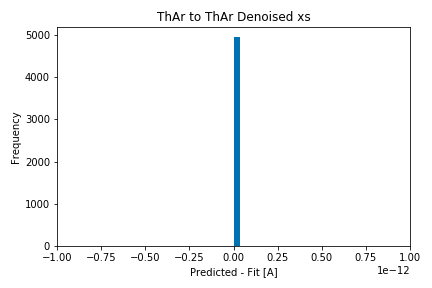
\includegraphics[width=0.48\textwidth]{Figures/tharTharDenoised.pdf}
\caption{Residuals for predicted wavelengths for the denoised x-values of an exposure used to train the PCA.   As expected, the residuals are zero within machine error for the case where LFCs are used and where ThArs are used.}
\label{fig:sanityTest}
\end{figure} 

We then predict wavelengths for the \textit{measured} line centers for an exposure that was used to construct the basis.  The linear interpolation in time should return identical PCA coefficients for this time.  Differences in wavelengths will arise from a combination of 1) noise in the measured line centers and 2) any interpolation error of lines to other x positions.  Figure \ref{fig:testHists} shows a histogram of the residuals for both the LFC (left) and the ThAr (right) in black.

\subsection{Training and Validation Tests} \label{sec:test-trainNvalid}
A more realistic test is to leave out some percentage of the calibration images from $\{exp_n\}$ while constructing the basis vectors and weights with PCA.  We then use the results from this PCA to predict wavelengths for lines in the calibrations images that were left out.  The used calibration images represent the ``training set," while the left out exposures make up the ``validation set."

We chose to use 90\% of available exposures to train the PCA, and leave the remaining 10\% for validation.  Exposures were sorted into either set at random.  \lz{(Worth including?) Because only two ThAr exposures were taken each night (at the very beginning and end), leaving ThAr exposures out often left just one ThAr exposure per night.  It was therefore impossible to run a similar test using just ThAr exposures.}

We are now also testing how well PCA coefficients are interpolated to other times outside of the training set, and, consequently, how well line centers can be reconstructed for all times.  As before, differences in wavelength will also be drawn from how well line centers are measured and error in interpolating to those measured values.  This second source of error was independently quantified in the second test described in the previous section.

\subsection{Cross Tests} \label{sec:test-cross}
Similar to the training and validation tests, we can also use one calibration source to construct the PCA basis and weights and the other to test the results.  We used LFC exposures to construct a wavelength solution, and then used it to predict wavelengths for measured line centers of ThAr lines.  We can then use the assigned wavelengths for each ThAr line to assess how well we predicted the wavelengths for these lines.  Likewise, we can use ThAr exposures to predict the wavelengths of LFC lines.

\begin{figure}[h]
\centering
\includegraphics[width=1\textwidth]{Figures/lfcgood.pdf}
\caption{Residuals from different wavelength calibration tests.  Left: residuals of wavelength predictions for LFC lines.  In black are the results from using all LFC exposures to construct a wavelength solution, and using it to predict wavelengths for the measured line centers of each exposure.  Over-plotted in blue are the residuals from the training and validation tests.
Right: residuals of wavelength predictions for ThAr lines or using ThAr lines.  The black histogram is the same as in the left plot, but with ThAr exposures instead of LFC exposures.  In blue is the residuals from using the LFC exposures to construct a wavelength solution that is then used to predict ThAr line wavelengths.  In green is using ThAr exposures to predict LFC line wavelengths. }
\label{fig:testHists}
\end{figure} 

Results from these tests are shown in Figure \ref{fig:testHists}.  The results of the self tests for LFC (left) and ThAr (right) exposures are shown as black outlines.  This histogram combines residuals from all exposures.  The self test represents the limit of how well the line centers at any given time can be predicted, since here we are predicting the line centers for an exposure used in the construction of $a_{nk}$.  \lz{How to quantify error from measurement of line center}.

Overplotted in the left plot of Figure \ref{fig:testHists} are the residuals from training the wavelength solution with only 90\% of LFC exposures and predicting the wavelengths for the remaining 10\% of exposures.  The two histograms match very closely, indicating that very little error is introduced when predicting denoised x values for times not used in the construction of the wavelength solution.

The right plot in \ref{fig:testHists} shows results involving the ThAr exposures.  Similar to with the LFC, the histogram of the ThAr self tests is shown in black, and provide a limit on how well lines at different times can be predicted.  If we use the LFCs, all taken at different times, to predict the ThAr lines, we see that again the histograms match very closely.  This confirms that interpolating $a_{nk}$ w.r.t. time is introducing little error.

Overplotted in green is the result from using ThAr lines to predict LFC line wavelengths.  These residuals show a scatter comparable to other results where the wavelength value of ThAr lines are being predicted.  This implies that using the ThAr to predict wavelengths is dominated by uncertainties in the measured line centers for the ThAr.
\lz{why is it skewed left a little??}

\section{Parametric Model} \label{sec:comparisons}
Classically, pipelines employ polynomials to construct smooth wavelength solutions for each exposure.  For example, the \expres\ pipeline described in \lz{Petersburg+} found the $\theta_{n}$ from equation 1 to be the amplitudes of some 2D, 9th-order polynomial in $x$ and $m$ for each $n$, making the equivalent to equation 2 the following:
\begin{equation}
\lambda(x,y,m,n) = \sum_{i=0}^9\sum_{j=0}^9 c_{nij}\, x^i\,m^j + \mathrm{noise}
\quad ,
\end{equation}
where the $c_{nij}$ are coefficients unique to exposure $n$.  These coefficients are then smoothed by a third-order polynomial over time.  This same polynomial was used to construct wavelengths for non-calibration exposures.
Coefficients, $c_{nij}$, were found that minimize an objective $Q$ that is something like the L2-norm:
\begin{equation}
Q = ||\lambda(x,y,m,n) - \sum_{i=0}^9\sum_{j=0}^9 c_{nij}\, x^i\,m^j||_2^2
\quad .
\end{equation}

Even in this simple context, where every calibration image $n$ is treated as its own unique flower, there are improvements to be made.
For one, the sums should not be from 0 to 9, but instead
\begin{equation}
\sum_{i=0}^9\sum_{j=0}^{9-i}
\quad ,
\end{equation}
because that is the definition of 9th order.  We find that fitting to 8th order is sufficient, faster, and leaves less residual pattern than the original 9th degree fit.

For another, the objective function could be made soft to permit catastrophic outliers without destroying the fit. (\lz{we did not do this}).  We might recommend the iteratively reweighted least squares (IRLS).  This would make the fitting more robust.

For yet another, there are rescaling issues for the products $x^i\,m^j$ to protect the fitting from near-singularities or bad conditioning of the linear-algebra operators.

\subsection{Comparisons}
To test each method, we took an LFC exposure and separated the even and odd lines.  We then used the even lines to predict wavelengths for the odd lines and vice versa.

For example, for the parametric model, we fit a 2D, 8th-degree polynomial to the odd lines.  We then evaluated this polynomial at the positions of the even lines to assign them wavelengths.  We then reversed the process by fitting a polynomial to the even lines and evaluating that polynomial at the positions of the odd lines.  Differences between the polynomial assigned wavelengths and the assigned wavelengths of each line are shown in Figure \ref{fig:dsnMFit}.

We run the test for both the original method described in \lz{Petersburg+}, but with an 8th degree polynomial rather than 9th, and changing the polynomial for the revised description of a 2D polynomial given in equation 5.  In the second case, the polynomial is also fit using a design matrix rather than by minimizing an objective (\lz{What's the fancier way of saying this}).  For the non-parametric model, we repeat the test using a cubic spline interpolator in place of a polynomial fit.

The results are shown in Figures \ref{fig:polyValFit}, \ref{fig:dsnMFit}, and \ref{fig:intpFit}.  Residuals for each line plotted with respect to order and x-pixel are shown on the left while the histogram of the residuals are shown on the right.  Moving from \lz{Petursburg+} to a design matrix polynomial fit with half the terms already reduces some of the correlated structure in the residuals that can be seen on the left in Figure \ref{fig:polyValFit}.  However, the same vertical stripes can be seen in the residuals for both methods.  This along with other evidence (outside the scope of this paper) suggests that these vertical stripes are due to defects present in the detector.

Using a non-parametric model, i.e. a cubic spline, gets rid of all correlated structure in the residuals and results in smaller residuals that are better centered around zero.  The non-parametric model was able to account for the high-order detector defects that are smoothed over by a polynomial fit, allowing for a more accurate fit.

\lz{Could (should) combine these three plots better.}

\begin{figure}[h]
\centering
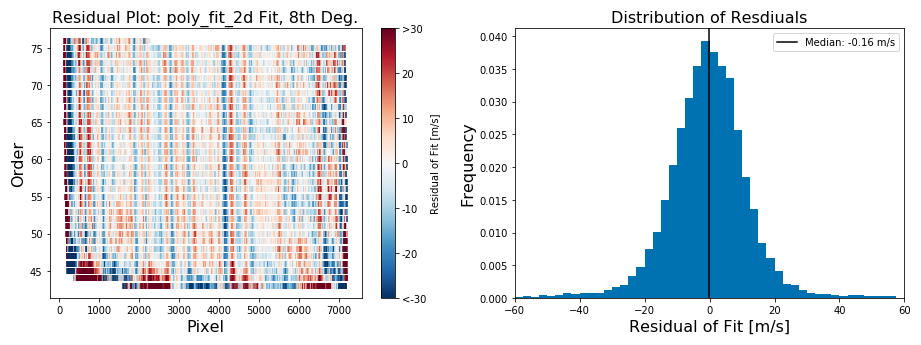
\includegraphics[width=\textwidth]{Figures/polyval2d.png}
%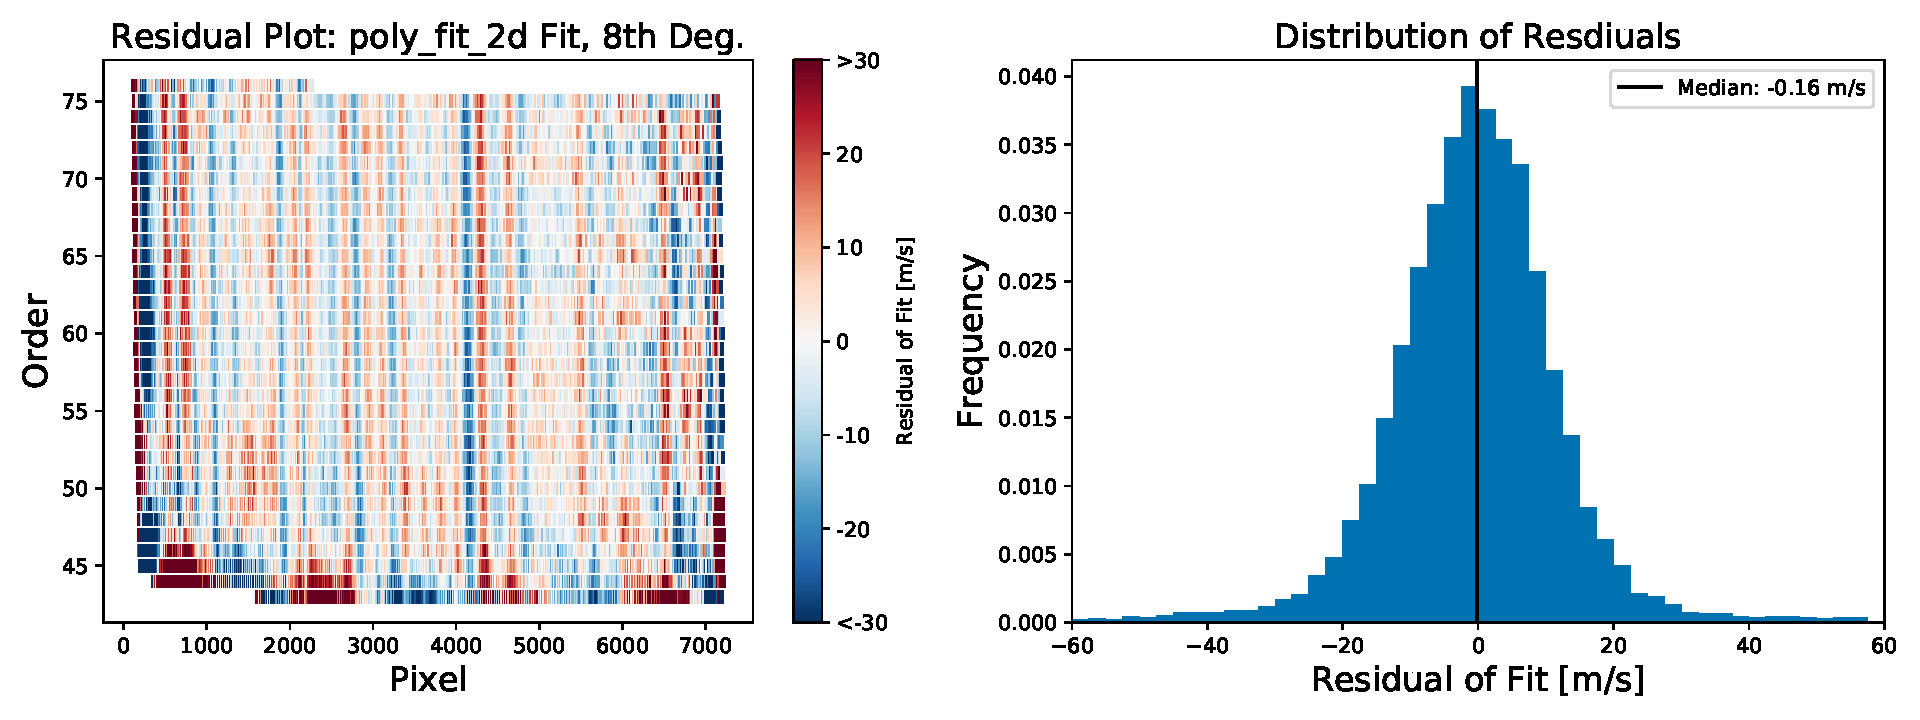
\includegraphics[width=\textwidth]{Figures/polyval2d.pdf}
\caption{\lz{Unclear whether it is worth a direct comparison with the old EXPRES pipeline} Residuals of a parametric model.  A 2D, 8th-degree polynomial fit was used to predict the wavelengths of each line.   Left shows the difference between the predicted and true wavelength for each line (color) across each order.  Right is a histogram of these residuals.  Residuals have been translated to velocity shifts.}
\label{fig:polyValFit}
\end{figure} 

\begin{figure}[h]
\centering
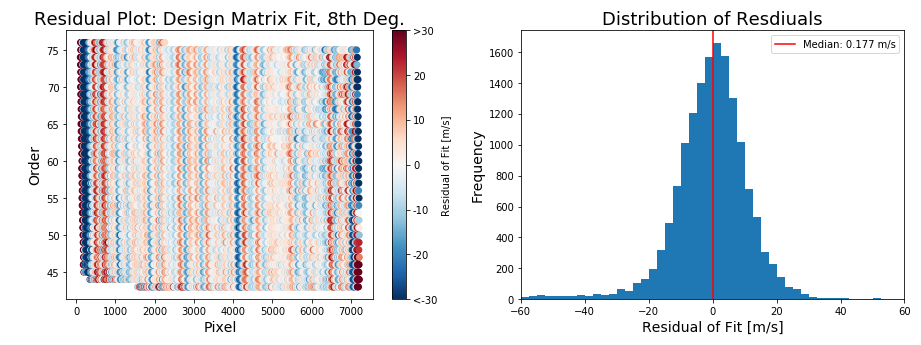
\includegraphics[width=\textwidth]{Figures/designMatrix.png}
%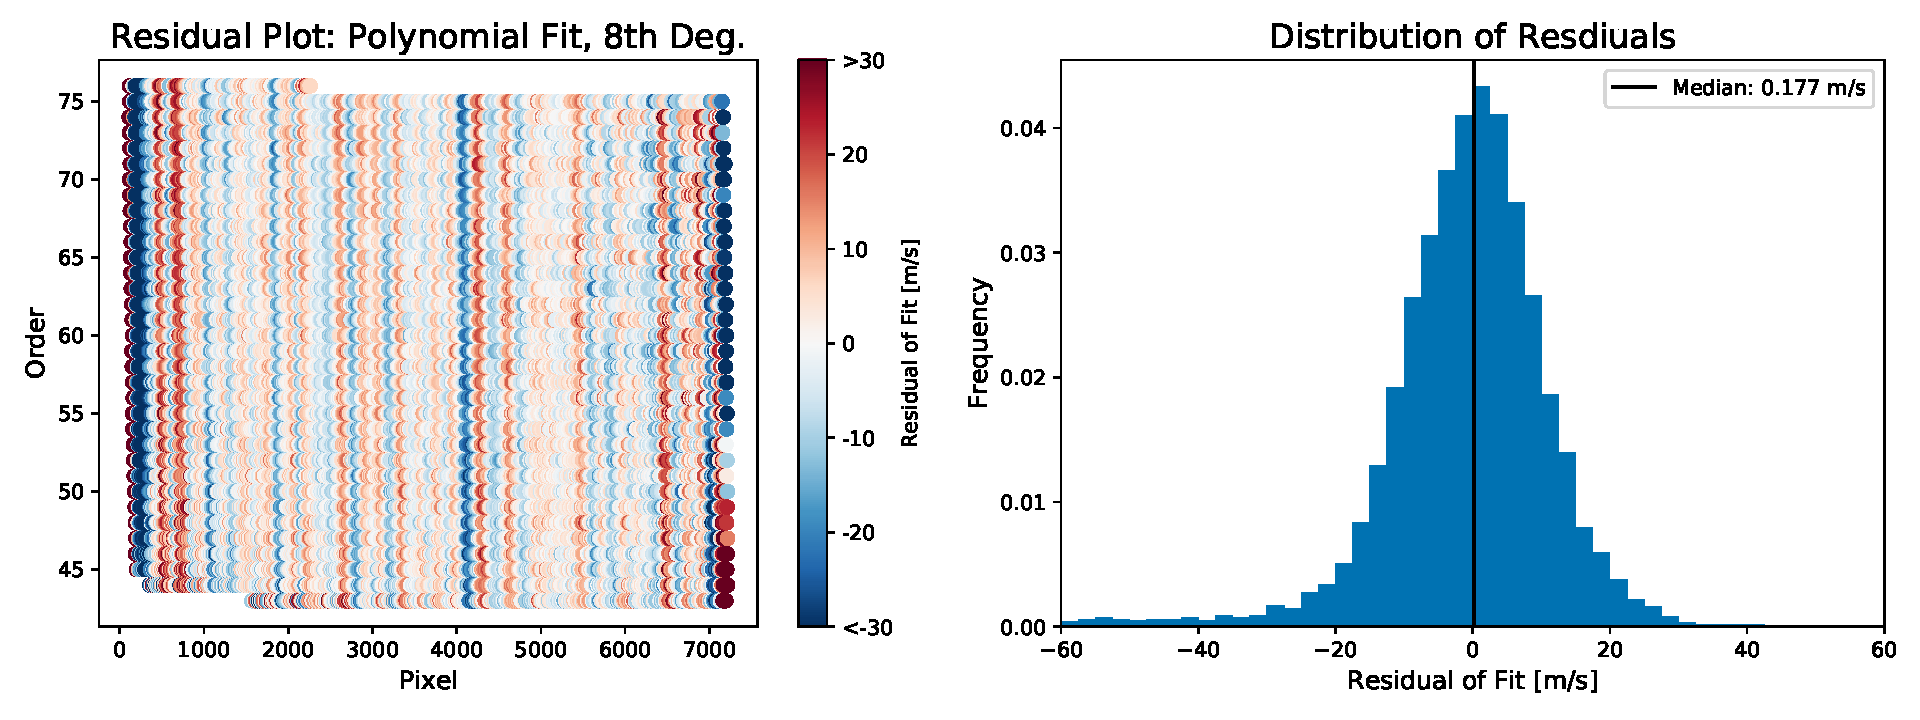
\includegraphics[width=\textwidth]{Figures/designMatrix.pdf}
\caption{Residuals of a parametric model fit using a design matrix.  A 2D, 8th-degree polynomial fit of the form given in equation 5 was used to predict the wavelengths of each line.  Otherwise, similar to Figure \ref{fig:polyValFit}.}
\label{fig:dsnMFit}
\end{figure} 

\begin{figure}[h]
\centering
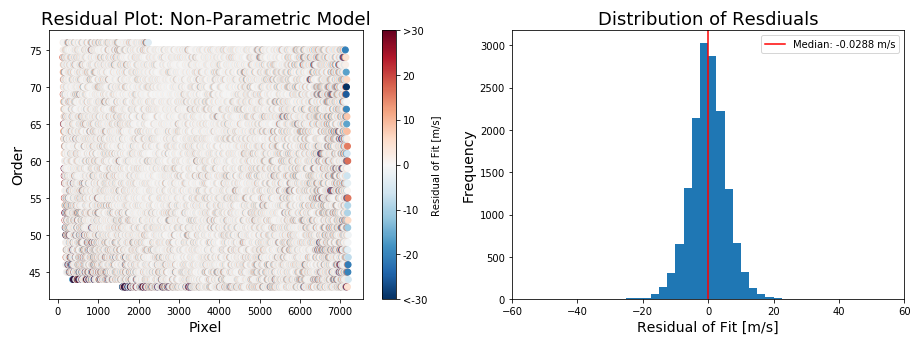
\includegraphics[width=\textwidth]{Figures/noHierc.png}
%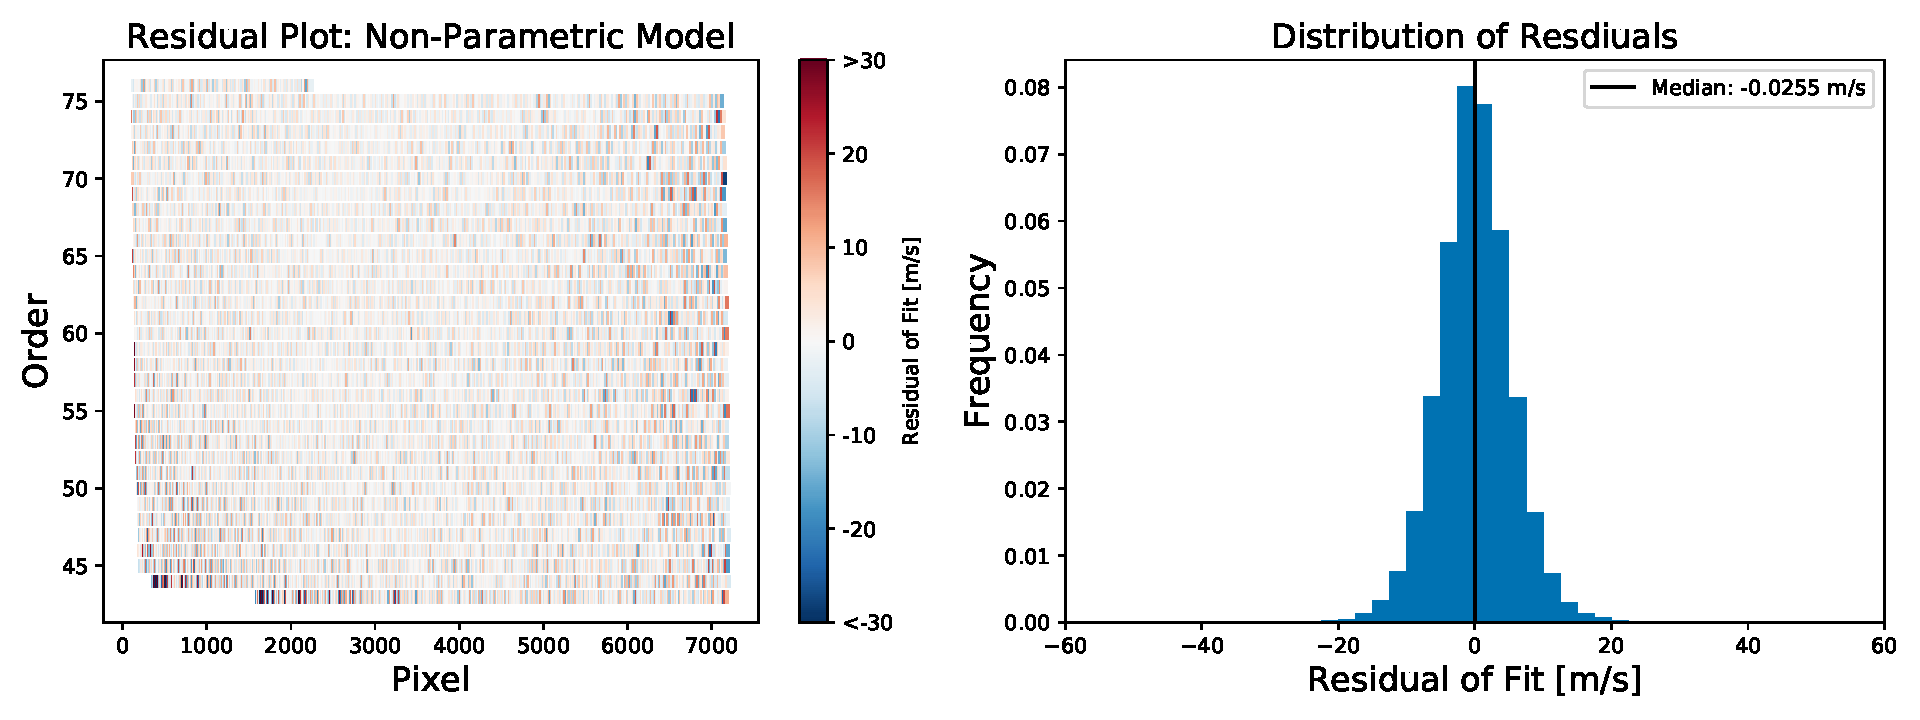
\includegraphics[width=\textwidth]{Figures/noHierc.pdf}
\caption{Residuals of a non-parametric model.  A PCHIP cubic spline interpolator was used to predict the wavelengths of each line.  otherwise similar to Figure \ref{fig:dsnMFit}.}
\label{fig:intpFit}
\end{figure} 

\section{Real Data Through to RVs} \label{sec:realdata}

\section{Discussion} \label{sec:discussion}

Practical statements?  How many exposures are needed to implement this method at all.  How often do exposures have to be taken throughout a night (unless that's too dependent on instrument stability)

Generalization to etalon:
All methods described here are easily adapted to use with an etalon or any other arc length for which a list of lines and their wavelengths can be constructed.

Self calibration idea:
Once we define a calibration space that captures all possible degrees of freedom for a stabilized spectrograph, then all exposures taken with the spectrograph contain information about where the spectrograph lies in that space at the time of the exposure.  Meaning, a science exposure can be used to determine the current state of the instrument in this calibration space.  It would therefore be possible to self-calibrate science exposures without the use of an additional wavelength calibration source.

Perfect degeneracy problem:
With any wavelength solution, there is a perfect degeneracy between what is defined as the ``center of the line'' and the resultant wavelength solution.  If, for example, a cross correlation method is used to extract RVs from the data, a systematic difference may be introduced depending on the definition of the center of the line.  In principle, the best way to mitigate this error would be to use a calibration source that looks like a star.


How hard would it be to go bayesian?

\end{document}
